\documentclass[11pt,letterpaper]{article}

\usepackage{hyperref}
\usepackage{graphicx}
\usepackage{fancybox}
\usepackage[utf8]{inputenc}
\usepackage{epsfig,graphicx}
\usepackage{multicol,pst-plot}
\usepackage{pstricks}
\usepackage{amsmath}
\usepackage{amsfonts}
\usepackage{amssymb}
\usepackage{eucal}
\usepackage{upgreek}
\usepackage[left=2cm,right=2cm,top=2cm,bottom=1cm]{geometry}
\usepackage{tcolorbox}
\usepackage{import}
\pagestyle{empty}
\DeclareMathOperator{\tr}{Tr}
\renewcommand{\sp}[1]{$${\begin{split}#1\end{split}}$$}

\usepackage{lipsum}
\usepackage{mdframed}
\usepackage{listings}
\usepackage{color}

% Margins
% \topmargin=-0.45in
\evensidemargin=0in
\oddsidemargin=0in
\textwidth=6.5in
\textheight=9.0in
\headsep=0.25in

 % The problem environment introduced.                                     
\newenvironment{problem}[2][Problem]                                  
        {\begin{tcolorbox}[colback=white,colframe=gray!50,title=#1 #2]}
        {\end{tcolorbox}}
        % {\begin{mdframed}[backgroundcolor=gray!20] \textbf{#1 #2} \\}
        % {\end{mdframed}}
% Define solution environment
\newenvironment{solution}                      
        {\begin{mdframed}\textit{Solution:} \\}
        {\end{mdframed}}
% Define an environments for proofs
\newenvironment{myproof} 
        {\textit{Proof:}}                                   
        {\begin{flushright} Q.E.D. \end{flushright}}
% Define a theorem environment and a notation one too
\newenvironment{mytheorem}                    
        {\begin{mdframed}\textbf{Theorem:} \\}
        {\end{mdframed}}
\newenvironment{notation}                      
        {\begin{mdframed}\textit{Notation:} \\}
        {\end{mdframed}}
% A new example wouldnt so any harm either...  
\newenvironment{example}                             
        {\textit{Example:}\\}
	{}
%I should be ashamed to forget the definition environment
\newenvironment{definition}
	{\begin{mdframed}$\underline{\textit{Def}^\textit{n}:} $\\}
	{\end{mdframed}}
%Corollary envvvvvvvvv
\newenvironment{corollary}
	{\textbf{Corrolary:}\\}

\pagestyle{empty}

\begin{document}

\begin{center}
  \Huge{JAVA Notes}\\
  \vspace{0.25cm}
  \small{Gurmukh Singh}
\end{center}

\vspace{-1.75cm}

\begin{flushright}
  Instructor: \\ Dr. Silky
\end{flushright}

\vspace{-1.3cm}

\begin{flushleft}
  B.Tech. CSE
\end{flushleft}

\rule{15.5cm}{0.1mm}%{\linewidth}{0.1mm}

% Optional TOC
\tableofcontents
\pagebreak

%--Paper--

\section{Introduction}
Java basics unit 1:
\begin{enumerate}
  \item Developed by Sun Microsystems in 1995
  \item Father of Java is James Gosling.
  \item It is high-level, robust, object oriented and secure. 
\end{enumerate}
Types of java applications:
\begin{itemize}
  \item Standalone applications. 
  \item Web applications. e.g. Servlet, JSP, Struts, Spring, Hibernate, JSF etc.
  \item Enterprise appliction. 
  \item Mobile application. e.g. Android and Java ME
\end{itemize}
Features of Java:
\begin{itemize}
  \item Simple.
  \item Object-oriented.(data and behavior)
  \item Automatic Garbage Collection.
  \item Platform-independent (Write once run anywhere WORA)
  \item Secure 
  \item Classloader
  \item Bytecode Verifier
\end{itemize}

Sidenote: We know that + adds numbers. we can also add objects with the help of the same operator by the help of operator overloading.

to Develop java applications you need JDK 
to Run java applications you need JRE

JRE is a part of JVM 

\subsection{Class loader}
\begin{enumerate}
  \item It is a part of JRE. It is used to load Java classes into the JVM.
  \item It adds \underline{security} by separating packages of local filesystem and those imported from network sources. 
\end{enumerate}

\subsection{Bytecode Verifier}
\begin{enumerate}
  \item It checks the code fragments for illegal code.
\end{enumerate}

\subsection{Security Manager}
\begin{enumerate}
  \item It determines what resources a class can access. e.g. reading and writing to the local disk.
\end{enumerate}
\begin{center}
  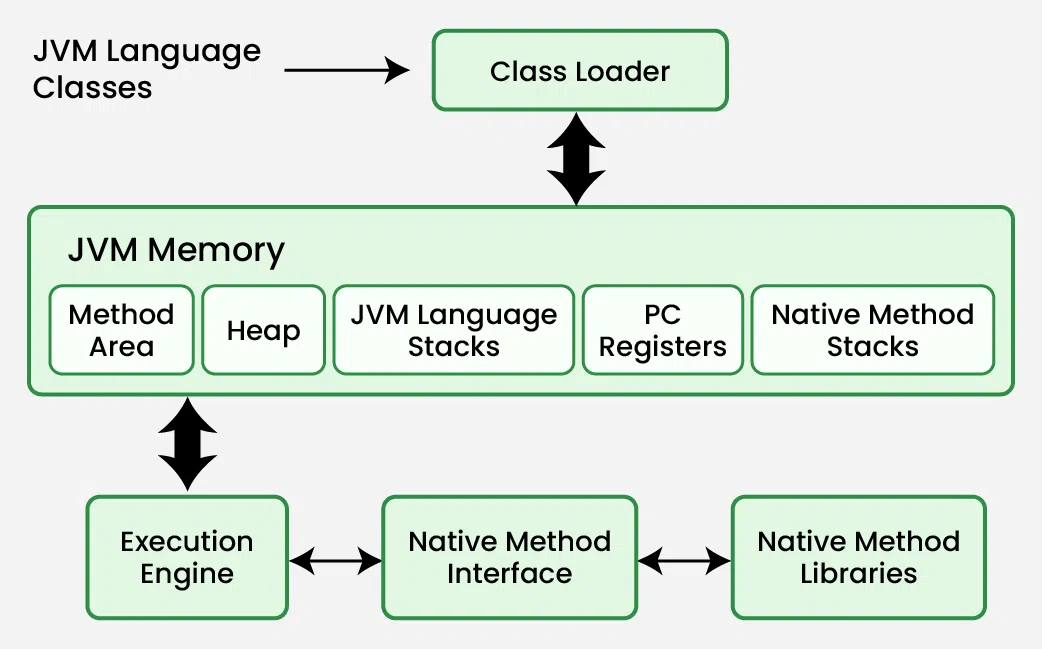
\includegraphics[width=\textwidth]{figs/JVM.png}
\end{center}
Sidenote: JVM Language stacks contain threads.

Homework: what is RMI and what EJB does
how to typecast
how is data loss handled in narrow casting

\subsection{Typecasting}
Assigning a value of 1 primite to another type is called typecasting. \\

\subsubsection{Widening cast(automatic)}
converting a smaller type to a larger type size.\\
byte $\rightarrow$ short $\rightarrow$ char $\rightarrow$ int $\rightarrow$ long $\rightarrow$ float $\rightarrow$ double 

\subsubsection{Narrowing cast(manual)}
converting a larger type to a smaller type size.\\
byte $\leftarrow$ short $\leftarrow$ char $\leftarrow$ int $\leftarrow$ long $\leftarrow$ float $\leftarrow$ double 

assinmen: if for while flowchart
\subsection{Operators}
\subsection{Variables}
There are three types of Variables. 
\begin{enumerate}
  \item Local Variable\\ 
    \begin{enumerate}
      \item A variable declared inside the body of the method is called local variable.
      \item A locar variable cannot be defined with "static" keyword. 
    \end{enumerate}
  \item Static variable.
    \begin{enumerate}
      \item It is something that belongs to the class.
      \item A variable that is declared as static is called a static variable. It cannot be local.
      \item A \underline{single copy} of the static variable is shared among all instances/objects of a class.
    \end{enumerate}
  \item Instance variable. 
    \begin{enumerate}
      \item A variable declared inside the class but outside th body of the methoud is called an instance variable. It is not declared as static.
    \end{enumerate}
\end{enumerate}

\begin{verbatim}
class student{
  int id;
  String name;
  static String college;
}
\end{verbatim}
The JVM allocates memory for method calls and local variables on the stack.\\
Stack memory is used for primited data types and references to objects\\
% TODO add the red diagram in the ppt
\end{document}
